\documentclass{beamer}
\usepackage[utf8]{inputenc}
\usepackage{amsmath}
\usepackage{mathtools}
\usepackage[greek]{babel}
\newcommand {\tl}{\textlatin}
\usepackage{tikz-cd}
\newcommand{\Gal}{\operatorname{Gal}}
\newcommand{\Q}{\mathbb{Q}}
\newcommand{\Z}{\mathbb{Z}}
\newcommand{\Lo}{\Lambda_{\mathcal{O}}}
\newcommand{\p}{\mathfrak{p}}
\newcommand{\q}{\mathfrak{q}}
\usepackage{tikz-cd}
\usepackage{verbatim}
\newtheorem{thrm}{Θεώρημα}
\newtheorem{lhmma}{Λήμμα}
\newtheorem{exa}{Παράδειγμα}
\newtheorem*{defn}{Ορισμός}
\newtheorem{prop}{Πρόταση}
\newtheorem{cor}{Πόρισμα}



\title{Μια Εισαγωγή στη Θεωρία \tl{Iwasawa}}
\author{Δημήτριος Νούλας }
\date{Δεκέμβριος 2022}


\mode<presentation>
{
  \usetheme{Copenhagen}
  % or ...

  \setbeamercovered{transparent}
  % or whatever (possibly just delete it)
}

\begin{document}

\maketitle

\AtBeginSection[]
{
  \begin{frame}<beamer>
    \frametitle{\tl{Outline}}
    \tableofcontents[currentsection]%,currentsubsection]
  \end{frame}
}

%\section{Προβλήματα που λύνει η Αλγεβρική Τοπολογία}
\setbeamercovered{invisible}

\begin{frame}
    
    \frametitle{Ομάδες Κλάσεων Iδεωδών}
    \begin{block}{Μια αναδρομή από αλγεβρική θεωρία αριθμών}
    $$6 = 2 \cdot 3 = (1-\sqrt{-5})(1+\sqrt{-5}) \in \mathbb{Z}[\sqrt{-5}]$$ Σε ιδεώδη:
    \begin{align*}
    (2)(3) &= (1-\sqrt{-5})(1+\sqrt{-5}) \\ 
    &= (2,1+\sqrt{-5})^2 (3,1+\sqrt{-5})(3,1-\sqrt{-5})
    \end{align*}

    $$2 \Z[\sqrt{-5}] = (2,1+\sqrt{-5})^2 \quad \quad  3\Z[\sqrt{-5}] = (3,1+\sqrt{-5})(3,1-\sqrt{-5})$$
    
\end{block}
\end{frame}

\begin{frame}
    %περιοχή Dedekind: όλα τα κλασματικά ιδεώδη είναι αντιστρέψιμα
    \frametitle{Ομάδες Κλάσεων Ιδεωδών}
    \begin{block}{Κλασματικά Ιδεώδη}
    π.χ. $$\frac{1}{3}   \mathbb{Z} \subseteq \mathbb{Q}$$
    Για $K$ σώμα αριθμών ο δακτύλιος ακεραίων $\mathcal{O}_K$ είναι περιοχή \tl{Dedekind}, δηλαδή όλα τα κλασματικά ιδεώδη είναι αντιστρέψιμα
    $$I \{x \in K: xI \subseteq \mathcal{O}_K\} = (1)$$

    $$C_K = \frac{\text{κλασματικά ιδεώδη}}{\text{κύρια ιδεώδη}}$$
    \pause

    \tl{Iwasawa}: $h_n = |C_K|$ κυρίως για $\Z_p$-επεκτάσεις.
    \end{block}
\end{frame}

\begin{frame}
\begin{block}{$P$-\tl{adic} $L$-\tl{functions}}
$$\chi: \Gal(\mathbb{Q}(\zeta_n)/\Q) \cong (\Z/n\Z)^\times \longrightarrow \mathbb{C}^\times$$
$$L(s,\chi) = \sum\limits_{n=1}^\infty \chi(n)n^{-s} = \prod\limits_{p} (1-\chi(p)p^{-s})^{-1} \quad \operatorname{Re}(s)>1$$
$$\prod\limits_{\substack{\chi \in X \\ \chi \neq 1} } L(1,\chi) = \frac{2^{r_1} (2\pi)^{r_2} R_K}{\omega_K \sqrt{|D_K|}} \cdot h_K$$

$$\mathcal{L}_p (1-n,\chi) = (1-\chi\omega^{-n}(p)p^{n-1})L(1-n,\chi\omega^{-n}) \quad n\geq 1$$
$$\prod\limits_{\substack{\chi \in X \\ \chi \neq 1}} \left(1-\frac{\chi(p)}{p}\right)^{-1} \mathcal{L}_p(1,\chi) = \frac{2^{n-1}R_p(K)}{\sqrt{\Delta_K}} \cdot h_K$$
\end{block}
\end{frame}


%\begin{frame}
%\frametitle{$L$-\tl{functions}}
%\begin{block}{Φιλοσοφία θεωρίας αριθμών:}
%$$X \longrightarrow L(s,X)$$

 

%Για $X = h_n$ κοιτάμε χαρακτήρες \tl{Dirichlet}:
%$$\chi: \Gal(\mathbb{Q}(\zeta_n)/\Q) \cong (\Z/n\Z)^\times \longrightarrow \mathbb{C}^\times$$

%$$L(s,\chi) = \sum\limits_{n=1}^\infty \chi(n)n^{-s} = \prod\limits_{p} (1-\chi(p)p^{-s})^{-1} \quad \operatorname{Re}(s)>1$$
%\end{block}
%\end{frame}

%\begin{frame}
%\frametitle{\tl{Local-Global Principle}}
%\begin{thrm}[\tl{Ostrowski}]
%Κάθε μη-τετριμμένη απόλυτη τιμή στο $\Q$ είναι ισοδύναμη είτε με την πραγματική απόλυτη τιμή $|\cdot |$ είτε με την $p$-αδική $|\cdot |_p$.

%$\Q \xhookrightarrow{} \Q_p$$
%$$\Q \xhookrightarrow{} \mathbb{R}$$
%\end{thrm}

%\end{frame}

%\begin{frame}
%\frametitle{\tl{Local-Global Principle}}
%\begin{block}{Παρεμβολή}
%Σταθεροποιούμε $\overline{\Q} \xhookrightarrow{} \mathbb{C}_p$.
%$$\omega : \mathbb{F}_p^\times \longrightarrow \Z_p^\times \subset \mathbb{C}_p$$ 
%$\omega(a)$ διακεκριμένη $(p-1)$-οστή ρίζα της μονάδας, με $\omega(a) \equiv a (\operatorname{mod}p)$.

 

%$$\mathcal{L}_p (1-n,\chi) = (1-\chi\omega^{-n}(p)p^{n-1})L(1-n,\chi\omega^{-n}) \quad n\geq 1$$


%\end{block}

%\end{frame}


%\begin{frame}
%\frametitle{\tl{P-adic L-functions}}

%\begin{block}{\tl{Dirichlet Class Number Formula}}
%Για $K$ αβελιανό σώμα αριθμών και $X$ η ομάδα χαρακτήρων που του αντιστοιχεί:
%$$\prod\limits_{\substack{\chi \in X \\ \chi \neq 1} } L(1,\chi) = \frac{2^{r_1} (2\pi)^{r_2} R_K}{\omega_K %\sqrt{|D_K|}} \cdot h_K$$

 

%Για $K$ πλήρως πραγματικό αβελιανό σώμα αριθμών, $[K:\Q] = n$ και $X$ η ομάδα χαρακτήρων που του αντιστοιχεί:

%$$\prod\limits_{\substack{\chi \in X \\ \chi \neq 1}} \left(1-\frac{\chi(p)}{p}\right)^{-1} \mathcal{L}_p(1,\chi) = \frac{2^{n-1}h_K R_p(K)}{\sqrt{\Delta_K}}$$


%\end{block}
%\end{frame}

%\begin{frame}
%\begin{align*}\{\text{Υποομάδες του } X \} &\longleftrightarrow \{\text{ Υποσώματα του } \Q(\zeta_n) \} \\
	%\Gal(K/\Q)^{\wedge} &\longleftrightarrow K \\
%Y &\longleftrightarrow \Q(\zeta_n)^{Y^{\perp}}
%\end{align*}

%\begin{figure}[H]
	%\centering
	%\begin{tikzcd}
		%\Q(\zeta_n)           & 1                                        & X=G^{\wedge}                                      \\
		%K \arrow[u, no head]  & H=\Gal(\Q(\zeta_n)/K) \arrow[u, no head] & H^{\perp} \cong (G/H)^{\wedge} \arrow[u, no head] \\
		%\Q \arrow[u, no head] & G \arrow[u, no head]                     & \{\chi_0\} = G^{\perp}  \arrow[u, no head]       
		%\end{tikzcd}
%\end{figure}

%\end{frame}

%\begin{frame}


%\begin{thrm}
%Αν $p|h^+_p$, τότε $p|h^-_p$. Ειδικότερα, $p|h_p$ αν και μόνο αν $p|B_m$ για κάποιο $m=2,4,\ldots, p-3$.
%\end{thrm}
%\begin{block}{}
%$$h_n^+: \quad \Q(\zeta_n + \zeta_n^{-1}) \subseteq \Q(\zeta_n)$$
%$$h_n^- := \frac{h_n}{h_n^+}$$
%$$\frac{t}{e^t-1} = \sum\limits_{m=0}^\infty B_m \frac{t^m}{m!}$$
%\end{block}
 
%\begin{block}{Εικασία \tl{Vandiver}}
%Για κάθε $p$ πρώτο αριθμό έχουμε $p\nmid h^+_p$. 
%\end{block}


%\end{frame}



\begin{frame}
\frametitle{$\Z_p$-Επεκτάσεις}
\begin{block}{Ύπαρξη}
$\Q_\infty \subseteq \Q(\zeta_{p^\infty})$:
$$\Gal(\Q_\infty/\Q) \cong \Z_p$$ και 
$$\Q_\infty = \cup_n \Q_n \quad \quad \Q_n:= \Q(\zeta_{p^{n+1}})^{(\Z/p\Z)^\times}$$ με 
$$\Gal(\Q_n/\Q) \cong \Z/p^n \Z$$

\pause

Για $K$ τυχαίο σώμα αριθμών $K_\infty = K\Q_\infty$
$$\Gal(K_\infty/K) \cong \Gal(\Q_\infty/\Q\cap K) \cong p^n \Z_p \cong \Z_p$$
$$K_n := K_\infty^{p^n \Z_p}$$
\end{block}
\end{frame}

\begin{frame}
\frametitle{Θεώρημα \tl{Iwasawa}}
\begin{thrm}
Έστω $K_\infty/K$ μια $\Z_p$-επέκταση και $h_n$ να είναι η τάξη της ομάδας κλάσεων του $K_n$. Αν $h_n = p^{e_n}r$ με  $(r,p)=1$, τότε υπάρχουν 
	ακέραιοι $\lambda \geq 0, \mu \geq 0, \nu$ και $n_0$ έτσι ώστε
	$$e_n = \lambda n + \mu p^n + \nu$$ για κάθε $n\geq n_0$, όπου τα $\lambda,\mu,\nu$ είναι όλα ανεξάρτητα του $n$. 
\end{thrm}

\pause

Ιδέα: $p$-\tl{Sylow} υποομάδα του $C_{K_n}$ ως πεπερασμένα παραγόμενο $\Lambda$-πρότυπο, όπου $\Lambda := \Z_p[[T]]$ η άλγεβρα του \tl{Iwasawa}.
\begin{itemize}
\item Αλγεβρική δομή των δακτυλίων $\Lo := \mathcal{O}_K[[T]]$ για $K/\Q_p$ πεπερασμένη επέκταση.
\item ((Κολλώντας)) την πληροφορία που δίνει η θεωρία κλάσεων σωμάτων σε κάθε πεπερασμένο στρώμα βλέποντας το $\Lambda$ ως προβολικό όριο ομαδοδακτυλίων.
\end{itemize}
\end{frame}

\begin{frame}
\frametitle{Θεωρία Κλάσεων Σωμάτων}

\begin{block}{Νόμος Αντιστροφής}
Έστω $K$ σώμα αριθμών, τότε υπάρχει το σώμα $H_K$ που είναι η μέγιστη αβελιανή αδιακλάδιστη επέκταση του $K$ και 
$$C_K \cong \Gal(H_K/K)$$

 

%$$\Q(\zeta_{p^\infty}) = \bigcup\limits_{n=1}^\infty \Q(\zeta_{p^n})$$
\end{block}

\end{frame}

\begin{frame}

\begin{prop}[Αλγόριθμος Διαίρεσης]
	Έστω $f,g \in \Lambda_{\mathcal{O}}$ με $f = a_0 + a_1 T + \cdots$ με $a_i \in \mathfrak{p} = (\pi)$ για κάθε $0\leq i \leq n-1$ και $a_n \in \mathcal{O}_K^\times$. Τότε υπάρχουν μοναδικά $q \in \Lo$ και $r \in \mathcal{O}_K [T]$ με βαθμό $\deg r\leq n-1$ έτσι ώστε

	$$g = qf + r$$
\end{prop}
\pause 
\begin{proof}
Τελεστής $\tau_n : \Lo \longrightarrow \Lo$
	$$b_0 + b_1 T + b_2 T^2 + \cdots \longmapsto b_n + b_{n+1}T + b_{n+2}T^2 + \cdots$$
    $$\tau_n(g) = \tau_n(qf)$$
\end{proof}

\end{frame}

\begin{frame}

\frametitle{\tl{Distinguished} Πολυώνυμα}
\begin{defn} Έστω $P(T) = T^n + a_{n-1}T^{n-1} + \cdots + a_1 T + a_0 \in \mathcal{O}_K[T]$. Θα λέμε το $P(T)$ είναι \tl{distinguished} αν $a_i \in (\pi)$ για τα $0\leq i \leq n-1$.
\end{defn}
\end{frame}

\begin{frame}
\frametitle{Θεώρημα Προπαρασκευής του \tl{Weierstrass}}

\begin{thrm}[\tl{p-adic Weierstrass Preparation Theorem}]
	Έστω $f(T) = \sum\limits_{i=0}^\infty a_i T^i \in \Lo$ και υποθέτουμε ότι υπάρχει $n \in \mathbb{N}$ με $a_i\in (\pi)$ για όλα τα $0\leq i \leq n-1$, ενώ $a_n \in \mathcal{O}^\times$. Τότε υπάρχει μοναδικό $U(T) \in \Lo$ αντιστρέψιμο και μοναδικό $P(T) \in \mathcal{O}[T]$ ένα \tl{distinguished} πολυώνυμο βαθμού $n$, έτσι ώστε
	$$f(T) = P(T)U(T).$$

	\noindent Αν το $f(T) \in \Lo$ είναι μη μηδενικό, τότε υπάρχει $\mu \in \Z, \mu \geq 0$ και $P(T) \in \mathcal{O}[T]$ \tl{distinguished} πολυώνυμο βαθμού 
	το πολύ $n$ και ένα αντιστρέψιμο $U(T)\in \Lo$ έτσι ώστε
	$$f(T) = \pi^{\mu} P(T) U(T).$$
\end{thrm}

\end{frame}

\begin{frame}
\frametitle{Αλγεβρική Δομή}
\begin{block}{Περιοχή Μοναδικής Παραγοντοποίησης}
$$\Lo: \text{\tl{UFD}}$$ 
$$\text{ανάγωγα:} \quad \pi, \text{ ανάγωγα \tl{distinguished} } P(T) \in \mathcal{O}[T]$$
$$\text{αντιστρέψιμα}: \quad U(T) \in \Lo^\times \text{ αν } U(0) \in \mathcal{O}^\times$$
\end{block}
\pause 

\begin{lhmma}
    Έστω $f,g \in \Lo$ σχετικά πρώτα. Τότε το ιδεώδες $(f,g)$ έχει πεπερασμένο δείκτη στο $\Lo$.
\end{lhmma}

\pause

\begin{lhmma}
    Έστω $f \in \Lo - \Lo^\times$. Τότε το $\Lo/(f)$ έχει άπειρη τάξη.
\end{lhmma}

\end{frame}


\begin{frame}
\frametitle{Αλγεβρική Δομή}


\begin{prop}
Οι πρώτοι του $\Lo$ είναι οι $0,(\pi,T),(\pi)$ και τα ιδεώδη $(P(T))$ όπου $P(T)$ είναι ανάγωγο \tl{distinguished} πολυώνυμο. Το ιδεώδες $(\pi,T)$ είναι το μοναδικό μέγιστο.
\end{prop}
\pause
\begin{proof}
    Έχουμε τους ισομορφισμούς:
    \begin{align*}
    \Lo/(\pi,T) &\cong \mathcal{O}/(\pi) \\
    \Lo/(\pi) &\cong (\mathcal{O}/(\pi))[[T]] \\
    \Lo/(P(T)) &\cong \mathcal{O}[T]/(P(T)) \\
    \Lo/0 &\cong \Lo ,
    \end{align*}
    Κάθε άλλη περίπτωση ανάγεται σε αυτές.
    \end{proof}

\end{frame}

\begin{frame}
\frametitle{Άλγεβρική Δομή}
\begin{lhmma}
    Έστω $f,g \in \Lo$ να είναι σχετικά πρώτα. Τότε
    \begin{enumerate}
        \item Η φυσική απεικόνιση
        $$\Lo/(fg) \longrightarrow \Lo/(f) \oplus \Lo /(g)$$ είναι μονομορφισμός με πεπερασμένο συνπυρήνα.
        \item Υπάρχει εμφύτευση
        $$\Lo/(f) \oplus \Lo/(g) \longrightarrow \Lo/(fg)$$ με πεπερασμένο συνπυρήνα.
    \end{enumerate}
\end{lhmma}
\end{frame}


\begin{frame}
\frametitle{Ψευδο-ισομορφισμός}
\begin{defn}
    Δύο $\Lo$-πρότυπα $M$ και $N$ θα λέγονται ψευδο-ισόμορφα και θα τα γράφουμε $M\sim N$, αν υπάρχει ακριβής ακολουθία:
    $$0 \longrightarrow A \longrightarrow M \longrightarrow N \longrightarrow B \longrightarrow 0$$ όπου τα $A,B$ είναι πεπερασμένα $\Lo$-πρότυπα.
\end{defn}
\pause
\begin{block}{Όχι Σχέση Ισοδυναμίας}
$$0 \longrightarrow (\pi,T) \longrightarrow \Lo \longrightarrow \mathcal{O}/(\pi)\longrightarrow 0$$ 
$$(\pi,T) \sim \Lo \ \text{ αλλά } \ \Lo \nsim (\pi,T).$$
\end{block}
\end{frame}


\begin{frame}
\frametitle{Θεώρημα Δομής}

\begin{thrm}[Δομής Πεπερασμένα Παραγόμενων $\Lo$-Προτύπων]
    Έστω $M$ ένα πεπερασμένα παραγόμενο $\Lo$-πρότυπο. Τότε
    $$M \sim \Lo^r \oplus \left(\bigoplus\limits_{i=1}^s \Lo/(\pi^{n_i})\right) \oplus \left( \bigoplus\limits_{j=1}^t \Lo/(f_j(T)^{m_j})\right)$$ όπου τα $r,s,t,n_i$ και $m_j$ ανήκουν στο $\Z$ και τα $f_j(T)$ είναι \tl{distinguished} και ανάγωγα πολυώνυμα. Αυτή η διάσπαση καθορίζεται πλήρως από το $M$.
\end{thrm}
\end{frame}

%\begin{frame}
%\frametitle{Θεώρημα Δομής}

%\begin{block}{Πράξεις}

%\textbf{Πράξη \tl{A}.} Μπορούμε να εναλλάσουμε τις γραμμές μεταξύ τους ή να εναλλάσουμε τις στήλες μεταξύ τους. \\
%\textbf{Πράξη \tl{B}.} Μπορούμε να προσθέσουμε ένα πολλαπλάσιο μιας γραμμής (ή στήλης) σε μια άλλη γραμμή (ή στήλη).\\
%\textbf{Πράξη \tl{C}.} Μπορούμε να πολλαπλασιάσουμε μια γραμμή ή στήλη με στοιχείο του $\Lo^\times$.


 
%\textbf{Πράξη 1.}  Αν το $R$ περιέχει γραμμή $(\lambda_1,\pi \lambda_2,\ldots, \pi \lambda_n)$ με $\pi \nmid \lambda_1$, τότε μπορούμε %να αλλάξουμε τον $R$ στον $R^\prime$, του οποίου η πρώτη γραμμή είναι $(\lambda_1,\lambda_2,\ldots,\lambda_n)$ και οι υπόλοιπες γραμμές %είναι οι γραμμές του $R$, όπου η πρώτη στήλη είναι πολλαπλασιασμένη με $\pi$.\\
%\textbf{Πράξη 2.} Αν όλα τα στοιχεία στην πρώτη στήλη του $R$ διαιρούνται από το $\pi^k$ και αν υπάρχει 
%γραμμή $(\pi^k\lambda_1,\ldots, \pi^k \lambda_n)$ με $\pi \nmid \lambda_1$, τότε μπορούμε να αλλάξουμε τον πίνακα στον 
%$R^\prime$ που είναι ο ίδιος με τον $R$, αλλά στην θέση της γραμμής $(\pi^k\lambda_1,\ldots, \pi^k \lambda_n)$ μπαίνει η 
%γραμμή $(\lambda_1,\ldots, \lambda_n)$.
%\noindent \textbf{Πράξη 3.} Αν το $R$ περιέχει γραμμή $(\pi^k \lambda_1,\ldots, \pi^k \lambda_n)$ και για κάποιο $\lambda \in \Lo$ με %$\pi\nmid \lambda$ η γραμμή $(\lambda \lambda_1,\ldots, \lambda \lambda_n)$ να είναι σχέση (όχι απαραίτητα γραμμή του $R$), τότε %μπορούμε να αλλάξουμε το $R$ με το $R^\prime$ που είναι το ίδιο εκτός από την γραμμή $(p^k \lambda_1,\ldots, \pi^k \lambda_n)$ που θα %αντικατασταθεί με την $(\lambda_1,\ldots, \lambda_n)$.


%\end{block}
%\end{frame}

\begin{frame}

\begin{block}{Στρώνουμε το έδαφος}
Έστω $K_\infty/K$ μια $\Z_p$-επέκταση, για κάθε $n \geq 1$ η επέκταση $K_\infty/K_n$ παραμένει $\Z_p$-επέκταση.
Θέτουμε $$\Gamma = \Gal(K_\infty/K) \cong \Z_p$$ και έστω $\gamma_0 \in \Gamma$ ένας τοπολογικός γεννήτορας.
$$x \in \Z_p \longmapsto \gamma_0^x\in \Gamma$$

\pause 

Έστω για κάθε $K_n$ θεωρούμε ως $L_n$ την μέγιστη αβελιανή αδιακλάδιστη $p$-επέκταση και θέτουμε $L= \cup_n L_n$ 
\pause

και
$$X = \Gal(L/K_\infty)$$
$$G = \Gal(L/K)$$

\end{block}
\end{frame}

\begin{frame}
\begin{block}{Στρώνουμε το έδαφος}
$$X_n = \Gal(L_n/K_n) $$
\pause είναι ισόμορφη με την $p$-\tl{Sylow} υποομάδα της $C_{K_n}$.

$ $\newline
Είτε ξεκινήσουμε από την $K_\infty/K$ ή την $K_\infty/K_n$ παίρνουμε το ίδιο $X$!

\end{block}
\end{frame}

\begin{frame}
\begin{lhmma}
Οι ομάδες διάσπασης και αδράνειας για άπειρη \tl{Galois} επέκταση είναι κλειστές ως προς την τοπολογία \tl{Krull}.
\end{lhmma}
\pause
Υπενθυμίζουμε ότι για μια άπειρη \tl{Galois} επέκταση $M/N$ λέμε ότι ένας πρώτος $\mathfrak{p}$ του $N$ διακλαδίζεται πλήρως αν υπάρχει μοναδικός πρώτος $\mathfrak{q}$ του $M$ έτσι ώστε $I_{\mathfrak q} = I_{\mathfrak q | \mathfrak p} = \Gal(M/N).$
$$\iff \mathfrak p \mathcal{O}_F = \mathfrak q_F^{[F:N]}$$
\pause 

\begin{prop}
    Κάθε $\Z_p$-επέκταση είναι αδιακλάδιστη έξω από το $p$, δηλαδή αν $\lambda$ είναι ένας πρώτος του $K$ που δεν στέκεται πάνω από το $p$, τότε η επέκταση $K_{\infty}/K$ είναι αδιακλάδιστη στο $\lambda$.
\end{prop}

\end{frame}

\begin{frame}
\begin{prop}
    Τουλάχιστον ένας πρώτος διακλαδίζεται στην επέκταση $K_\infty/K$ και υπάρχει $m\geq 0$ τέτοιο ώστε κάθε πρώτος που διακλαδίζεται στην επέκταση $K_\infty/K_m$ να διακλαδίζεται πλήρως.
\end{prop}

\pause
\begin{prop}
        Για κάθε $n\geq m$ έχουμε ότι $K_{n+1}\cap L_n = K_n$.
    \end{prop}
\pause
$$\Gal(L_nK_{n+1}/K_{n+1}) \cong \Gal(L_n/K_n)$$
$$L_n K_{n+1} \subset L_{n+1}$$
$$X_{n+1} \longrightarrow X_n$$
$$X_n = \Gal(L_n/K_n) \cong \Gal(L_nK_\infty/K_\infty)$$

\end{frame}

\begin{frame}
\begin{align*}
    \varprojlim X_n &= \varprojlim \Gal(L_n/K_n) \\
    &\cong  \varprojlim \Gal(L_n K_\infty/K_\infty) \\
    &\cong \Gal \left( \bigcup\limits_n\left(L_n K_\infty\right)/K_\infty \right) \\
    &= \Gal(L/K_\infty) \\
    &= X
\end{align*}
\pause 
\begin{block}{Δράση Συζυγίας}
$$\Gamma_n := \Gamma/\Gamma^{p^n} \cong \Z/p^n\Z \cong \Gal(K_n/K)$$
$$\gamma_n \in \Gamma_n \text{ δρα στο } X_n \text{ εφόσον ανυψώσουμε σε } \tilde{\gamma}_n \in \Gal(L_n/K)$$

$$\gamma_n \cdot x_n = \tilde{\gamma}_n x_n \tilde{\gamma}_n^{-1}$$
$$\text{Το } X_n \text{ γίνεται } \Z_p[\Gamma_n]\text{-πρότυπο}$$
\end{block}

\end{frame}

\begin{frame}
\begin{thrm}
$$\Lambda = \Z_p[[T]] \cong \varprojlim \Z_p[\Gamma_n] = : \Z_p [[\Gamma]]$$
$$1+T \longleftrightarrow \gamma_0$$
\end{thrm}

\pause
\begin{proof}
    $$\Gamma = \Gal(K_\infty/K) \cong \varprojlim \frac{\Gal(K_\infty/K)}{\Gal(K_\infty/K_n)} \cong \varprojlim \Gal(K_n/K) \cong \varprojlim \Gamma_n$$ 

    $$\Z_p[\Gamma_n] \cong \frac{\Z_p[T]}{\left((1+T)^{p^n}-1\right)} \cong \frac{\Z_p[[T]]}{\left((1+T)^{p^n}-1\right)}$$

    $$\Z_p[[T]] \cong \varprojlim \frac{\Z_p[T]}{\left(p,T\right)^n}$$
\end{proof}
\end{frame}

\begin{frame}
\begin{block}{Δράση Συζυγίας}
$$\Lambda \cong \varprojlim \Z_p[\Gamma_n]$$ δρα στο
$$X \cong \varprojlim X_n$$
((κατά συντεταγμένη)), δηλαδή για $\gamma \in \Gamma$ και $x \in X$


$$\gamma \cdot x = \tilde{\gamma} x \tilde{\gamma}^{-1}$$
όπου ανυψώνουμε σε $\tilde{\gamma} \in \Gal(L/K_m)$ για το $m$ από πριν.

$$X \text{ είναι } \Lambda\text{-πρότυπο}$$
\end{block}

\end{frame}

\begin{frame}
\frametitle{$X_n$ ως πηλίκο του $X$}

Θεωρούμε ότι $m=0$.
\begin{block}{Βάση Επαγωγής}
 $\mathfrak{p}_1,\ldots , \p_s$ οι πρώτοι που διακλαδίζονται στην επέκταση $K_\infty/K$. Σταθεροποιούμε έναν πρώτο $\q_i$ του $L$ που στέκεται πάνω από το $\p_i$.

 $$I_i = I(\q_i \mid \p_i), \quad L/K_\infty \text{ αδιακλάδιστη }$$
 $$I_i \cap X = 1$$
 $$I_i \xhookrightarrow{} G/X \cong \Gamma \text{ επιμορφισμός }$$
 $$G = I_i X = X I_i$$
 $$\gamma_0 \longleftrightarrow \sigma_i \in I_i, \quad  \sigma_i = a_i \sigma_1, \quad  a_i \in X$$
\end{block}
\end{frame}

\begin{frame}
\frametitle{$X_n$ ως πηλίκο του $X$}
\begin{lhmma}$$[G,G] = (\gamma_0 -1) \cdot X = TX$$
\end{lhmma}
\begin{block}{Βάση Επαγωγής}
Θέτουμε $Y_0$ να είναι το $\Z_p$-υποπρότυπο του $X$ που παράγεται από τα $TX$ και $\{a_i: \ 2\leq i \leq s\}$.
$$\nu_n := 1 + \gamma_0 + \cdots + \gamma_0^{p^n-1} = \frac{\gamma_0^{p^n}-1}{\gamma_0 -1 } = \frac{(1+T)^{p^n}-1}{T}$$

$$Y_n = \nu_n \cdot Y_0$$




\end{block}
\end{frame}

\begin{frame}
\frametitle{$X_n$ ως πηλίκο του $X$}
\begin{lhmma}
    Για $n\geq 0$ έχουμε
    $$X_n \cong X/Y_n$$
\end{lhmma}
\pause 
\begin{proof}
\begin{align*}
        X_0 &= \Gal(L_0/K) \\
        &= G/Gal(L/L_0) \\
        &= XI_1 / \overline{\langle (\gamma_0-1)\cdot X, a_2,\ldots,a_s,I_1\rangle}\\
        &\cong X/\overline{\langle (\gamma_0-1)\cdot X,a_2,\ldots,a_s\rangle} \\
        &= X/Y_0
    \end{align*}
    αλλαγές: $\sigma_i \rightarrow \sigma_i^{p^n}, \ a_i \rightarrow \nu_n \cdot a_i$, $$(\gamma_0-1)X \rightarrow (\gamma_0^{p^n}-1)X = \nu_n(\gamma_0-1)X$$
\end{proof}

\end{frame}

\begin{frame}
\frametitle{$X$ πεπερασμένα παραγόμενο $\Lambda$-πρότυπο}
\begin{lhmma}
Έστω $M$ ένα συμπαγές $\Lambda$-πρότυπο. Αν το $M/(p,T)M$ είναι πεπερασμένα παραγόμενο, τότε το $M$ είναι πεπερασμένα παραγόμενο $\Lambda$-πρότυπο.
\end{lhmma}
\pause 
\begin{cor}
    Το $\Lambda$-πρότυπο $X= \Gal(L/K_\infty)$ είναι πεπερασμένα παραγόμενο.
\end{cor}
\pause
\begin{proof}$$\nu_1 = ((1+T)^p -1)/T \in (p,T)$$
$$Y_0/(p,T)Y_0 \text{ πηλίκο του } Y_0/\nu_1 \cdot Y_0 = Y_0/Y_1 \subset X/Y_1 = X_1$$
$$\implies Y_0 \text{ πεπερασμένα παραγόμενο }, \quad  X/Y_0 = X_0$$
$$\implies X \text{ πεπερασμένα παραγόμενο }$$
\end{proof}

\end{frame}

\begin{frame}
\frametitle{$X_n$ ως πηλίκο του $X$}
\begin{block}{Διόρθωση}
\begin{align*} 
    \nu_{n,m} &= \frac{\nu_n}{\nu_m} \\
    &= 1+\gamma_0^{p^m} + \gamma_0^{2p^m} + \cdots + \gamma_0^{p^n - p^m}.
\end{align*} Εφόσον $\Gal(K_\infty/K_m) \cong \Gamma^{p^m}$ παράγεται από $\gamma^{p^n}$.
\end{block}
\pause
\begin{lhmma}
Έστω $K_\infty/K$ μια $\Z_p$-επέκταση. Το $X$ είναι πεπερασμένα παραγόμενο $\Lambda$-πρότυπο και υπάρχει $m\geq 0$ τέτοιο ώστε
    $$X_n \cong X/\nu_{n,m} Y_m$$ για κάθε $n\geq m$, όπου το $Y_m$ είναι αυτό που έχει οριστεί προηγουμένως.
\end{lhmma}


\end{frame}

\begin{frame}
\frametitle{Θεώρημα Δομής}
\begin{block}{Δομή του $X$}
    $$X/Y_m \cong \frac{X_m}{Y_m/\nu_{n,m}Y_m}\text{ πεπερασμένο} $$
    $$Y_m \sim X \sim \Lambda^r \oplus \left( \bigoplus \Lambda/(p^{\mu_i})\right) \oplus \left(\bigoplus \Lambda/(f_j(T)^{m_j})\right)$$
    Υπολογίζουμε την τάξη του $M/\nu_{n,m}M$ για κάθε συνιστώσα $M$.
    \pause 
    $$\begin{cases}
    M = \Lambda: & \Lambda/(\nu_{n,m}) \text{ άπειρο } \implies r= 0. \\ 
    M = \Lambda/(p^k): & \Lambda/(p^k, \nu_{n,m}) \implies (p^k)^{p^n-p^m} = p^{kp^n + c} \\
    M = \Lambda/(f(T)^k): & p^{dn+c}, \ d = \deg f(T)^r, n > n_0
    \end{cases}$$
\end{block}
\end{frame}

\begin{frame}

\begin{prop}
    Υποθέτουμε ότι 

    $$N = \Lambda^r \oplus \left( \bigoplus \Lambda/(p^{\mu_i})\right) \oplus \left(\bigoplus \Lambda/(f_j(T))\right),$$ όπου κάθε $f_j$ είναι \tl{distinguished}. Έστω $\mu = \sum \mu_i$ και $\lambda = \sum \deg f_j$. Αν το $N/\nu_{n,m}N$ είναι πεπερασμένο για κάθε $n$, τότε $r=0$ και υπάρχουν $n_0$ και $c$ έτσι ώστε

    $$|N/\nu_{n,m}N| = p^{\mu p^n + \lambda n + c}$$ για κάθε $n\geq n_0$.
\end{prop}
\end{frame}
\begin{frame}
\begin{block}{Πρόβλημα}
$$\text{Ξέρουμε την τάξη του } N/\nu_{n,m}N \quad \forall n \geq n_0$$
$$Y_m \sim N$$

$$\text{Θέλουμε την τάξη του } Y_m/\nu_{n,m}Y_m \quad \forall n \geq n_0$$
\end{block}
\pause
\begin{lhmma}
    Έστω $M$ και $N$ να είναι $\Lambda$-πρότυπα με $M\sim N$ και το $M/\nu_{n,m}M$ να έχει πεπερασμένη τάξη για κάθε $n\geq m$. Για κάποιο σταθερό $a$ και κάποιο $n_0$ έχουμε
    $$ |M/\nu_{n,m}M| = p^a |N/\nu_{n,m}N|$$ για κάθε $n\geq n_0$. 
\end{lhmma}

\end{frame}

\begin{frame}
\[
\centering
\begin{tikzcd}[ampersand replacement=\&, column sep=small]
            \& 0 \arrow[d]                                        \& 0 \arrow[d]                        \& 0 \arrow[d]                                                 \&   \\
            \& \ker \phi^\prime_n \arrow[d]                       \& \ker\phi \arrow[d]                \& \ker \phi^{\prime\prime}_n \arrow[d]                        \&   \\
0 \arrow[r] \& {\nu_{n,m} M} \arrow[d, "\phi^\prime_n"] \arrow[r] \& M \arrow[r] \arrow[d, "\phi"]      \& {M/\nu_{n,m}M} \arrow[r] \arrow[d, "\phi^{\prime\prime}_n"] \& 0 \\
0 \arrow[r] \& {\nu_{n,m}N} \arrow[d] \arrow[r]                   \& N \arrow[r] \arrow[d]              \& {N/\nu_{n,m}N} \arrow[r] \arrow[d]                          \& 0 \\
            \& \operatorname{coker}\phi^\prime_n \arrow[d]       \& \operatorname{coker}\phi \arrow[d] \& \operatorname{coker}\phi^{\prime\prime}_n \arrow[d]         \&   \\
            \& 0                                                  \& 0                                  \& 0                                                           \&  
\end{tikzcd}
\]

\end{frame}

\begin{frame}
\begin{thrm}[\tl{Iwasawa}]
	Έστω $K_\infty/K$ μια $\Z_p$-επέκταση και $h_n$ να είναι η τάξη της ομάδας κλάσεων του $K_n$. Αν $h_n = p^{e_n}r$ με  $(r,p)=1$, τότε υπάρχουν 
	ακέραιοι $\lambda \geq 0, \mu \geq 0, \nu$ και $n_0$ έτσι ώστε
	$$e_n = \lambda n + \mu p^n + \nu$$ για κάθε $n\geq n_0$, όπου τα $\lambda,\mu,\nu$ είναι όλα ανεξάρτητα του $n$. 
\end{thrm}

\begin{proof}
\begin{align*}
    p^{e_n} &= |X_n| \\
    &= |X/Y_m|\cdot |Y_m/\nu_{n,m}Y_m| \\
    &=p^b \cdot |N/\nu_{n,m}N| \\ 
    &= p^{\lambda n + \mu p^n + \nu}
\end{align*} για κάθε $n\geq n_0$. 
\end{proof}
\end{frame}

\begin{frame}
\begin{block}{$p$-αδικός χαρακτήρας \tl{Artin}}
Συνεχής ομομορφισμός ομάδων με πεπερασμένη εικόνα:
$$\chi : \Gal(F^{\operatorname{sep}}/F) \longrightarrow \overline{\Q}_p^\times$$
$$\chi: \Gal(F^\chi/F) \longrightarrow \left< \zeta_n \right> \subseteq \overline{\Q}_p^\times$$ 

Τύπου \tl{S} αν $F^\chi \cap F_\infty = F$. \\
Τύπου \tl{W} αν $F^\chi \subset F_\infty$.
$$F^\chi_\infty = F_\infty F^\chi = \cup_n F^\chi_n$$
Αν $\chi$ τύπου \tl{S} τότε έχουμε τους ισομορφισμούς:
$$\Gamma = \Gal(F^\chi_\infty/F^\chi) \longrightarrow \Gal(F_\infty/F)\cong \Z_p$$ 
$$\Delta = \Gal(F^\chi_\infty/F_\infty) \longrightarrow \Gal(F^\chi/F)$$




\end{block}
\end{frame}

\begin{frame}

\[
\centering
\begin{tikzcd}[ampersand replacement=\&, column sep=small]
        \& F^\chi_\infty                                      \&                                         \\
F^\chi \arrow[ru, "\Gamma", no head] \&                                                    \& F_\infty \arrow[lu, "\Delta"', no head] \\
        \& F \arrow[ru, "\Z_p"', no head] \arrow[lu, no head] \&                                        
\end{tikzcd}
\]

\begin{block}{Όμοια με πριν}
$L_n$ μέγιστη αδιακλάδιστη αβελιανή $p$-επέκταση του $F_n^\chi$. $X_n = \Gal(L_n/F^\chi_n)$ ισόμορφο με την $p$-\tl{Sylow} υποομάδα της ομάδας κλάσεων του $F^\chi_n$.\\
$$L = \cup L_n F^\chi_\infty$$
$$X \cong \varprojlim X_n $$
\end{block}
\end{frame}


\begin{frame}

\[
\centering
    \begin{tikzcd}[ampersand replacement=\&, column sep=small]
        \&                                                                          \& L                                                                         \&                                                          \&                                         \\
        \& L_n \arrow[ru, no head]                                                  \&                                                                           \& F^\chi_\infty \arrow[lu, "X"', no head]                  \&                                         \\
L_0 \arrow[ru, no head] \&                                                                          \& F_n^\chi \arrow[lu, "X_n"', no head] \arrow[ru, "\Gamma^{p^n}"', no head] \&                                                          \& F_\infty \arrow[lu, "\Delta"', no head] \\
        \& F^\chi \arrow[lu, "X_0", no head] \arrow[ru, "\Gamma/\Gamma^{p^n}"', no head] \&                                                                           \& F_n \arrow[ru, "p^n \Z_p"', no head] \arrow[lu, no head] \&                                         \\
        \&                                                                          \& F \arrow[ru, "\Z/p^n\Z"', no head] \arrow[lu, no head]                    \&                                                          \&                                        
\end{tikzcd}
\]

\begin{block}{$X$ ως $\Z_p[[\Gamma]]$-πρότυπο}
$$\Gamma \times \Delta \text{ δρα με συζυγίες στο } X$$
$$X \text{ γίνεται } \Z_p[[\Gamma \times \Delta]]-\text{πρότυπο} $$
\end{block}
\end{frame}

\begin{frame}
\begin{block}{Θεώρημα Δομής}
    $$X \sim \left(\bigoplus\limits_i \Lambda/(p^{\mu_i})\right) \oplus \left(\bigoplus\limits_j \Lambda/(f_j(T)^{m_j})\right)$$
\end{block}
$$V = X \otimes_{\Z_p} \overline{\Q}_p \cong \bigoplus \overline{\Q}_p [T]/(f_j(T)^{m_j})$$
$$f_X(T) = \prod f_j(T)^{m_j}$$ χαρακτηριστικό πολυώνυμο της δράσης του $\gamma_0 -1$ στο $V$.
$$V = \bigoplus\limits_{\psi \in \Delta^\wedge} \varepsilon_\psi V \quad \text{ ως } \overline{\Q}_p [\Delta]\text{-πρότυπο}$$
$$V^\chi := \varepsilon_\chi V = \{v\in V: \sigma v = \chi(\sigma)v \ \forall \sigma \in \Delta\}$$
$$f_\chi(T) \text{ χαρακτηριστικό πολυώνυμο της δράσης του } \gamma_0 -1 \text{ στο } V^\chi$$


\end{frame}

\begin{frame}
\begin{block}{\tl{P. Deligne} \& \tl{K. Ribet}}
Έστω $\psi$ χαρακτήρας του $F$ τέτοιος ώστε το $F^\psi$ να είναι πλήρως πραγματικό. Τότε υπάρχει η αντίστοιχη $p$-αδική $L$-συνάρτηση $\mathcal{L}_p(s,\psi)$.
$$H_\psi(T) = \begin{cases}
    \psi(\gamma_0)(1+T)-1, & \psi \text{ είναι τύπου } W \text{ ή τετριμμένο}, \\
    1, & \text{ διαφορετικά. }
\end{cases}$$ Για $\mathcal{O}_\psi := \Z_p[\psi]$ υπάρχει $G_\psi(T) \in \mathcal{O}_\psi [[T]]$ έτσι ώστε
$$\mathcal{L}_p (1-s,\psi) =\frac{ G_\psi ((1+p)^s -1)}{H_\psi((1+p)^s -1)}$$
$$\rho \text{ χαρακτήρας τύπου \tl{W}: } \  G_{\psi \rho}(T) = G_\psi(\rho(\gamma_0)(1+T)-1)$$
$$\chi\text{ περιττός, } \psi = \chi^{-1} \omega $$
$$\text{ Θ. Προπαρασκευής: } G_\psi((1+p)(1+T)^{-1}-1) =  \pi^{\mu_\chi} g_\psi(T)u_\psi(T)$$


\end{block}
\end{frame}

\begin{frame}
\begin{thrm}[Κύρια Εικασία της Θεωρίας \tl{Iwasawa}]
Για $\chi$ περιττό χαρακτήρα τύπου \tl{S} και $p$ έναν περιττό πρώτο έχουμε

    $$f_\chi(T) = g_{\chi^{-1}\omega}(T)$$
\end{thrm} \pause

\begin{figure}[H]
\centering
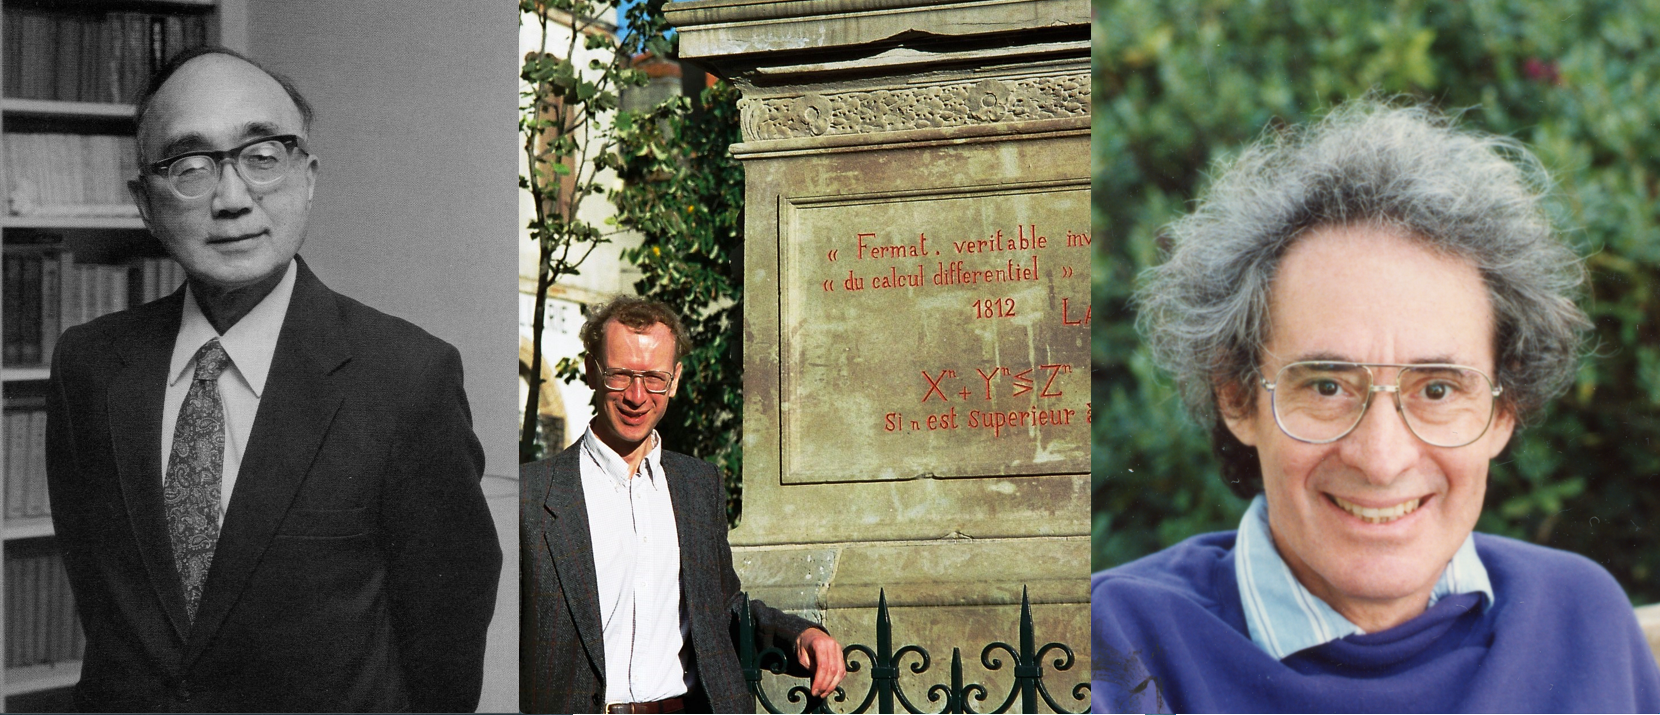
\includegraphics[scale=0.25]{iwasawa_wiles_mazur}
\end{figure}

\end{frame}

%\begin{frame}
%\frametitle{Μια Εισαγωγή στη Θεωρία \tl{Iwasawa}}

%\begin{block}{\centering Σας ευχαριστώ πολύ!}
%\end{block}
%\end{frame}

\begin{frame}
\frametitle{Σας ευχαριστώ πολύ!}
\begin{block}{Απόσπασμα από το \tl{Fermat's Last Theorem} του \tl{Simon Singh}}
\selectlanguage{english}
{\em Iwasawa theory on its own had been inadequate. The Kolyvagin-Flach method on its own was also inadequate. Together they complemented each other perfectly. It was a moment of inspiration that Wiles will never forget. As he recounted these moments the memory was so powerful that he was moved to tears: "It was so indescribably beautiful; it was so simple and so elegant. I couldn't contain myself, I was so excited. It was the most important moment of my working life. Nothing I ever do again will mean as much."}
\end{block}
\end{frame}




\end{document}